\documentclass{article}

\usepackage[utf8]{inputenc}
\usepackage{graphicx}

\title{Assignment on TWI Communication}
\author{Mahdi Hasnat Siyam , 1705003}
\begin{document}

\maketitle

% \tableofcontents

\section{Brief Introduction of the Two-Wire Interface}
TWI is serial , synchronous , bidirectional ,
multi-master , and self-reserved communication bus.
It has two wire namely SDA and SCL.
SDA is serial data line and SCL is serial clock line.
\subsection{Properties of TWI}
\begin{itemize}
	\item Both SDA and SCL are connected to power 
	source with pull up resistor. So devices can force voltage of SDA, SCl to low only.
	\item There are $7$ bit for address. 
	So total of $2^7 = 128$ distinct addressable devices can communicate via this interface.

	\item 
	\begin{figure*}[h!]
		\centering
		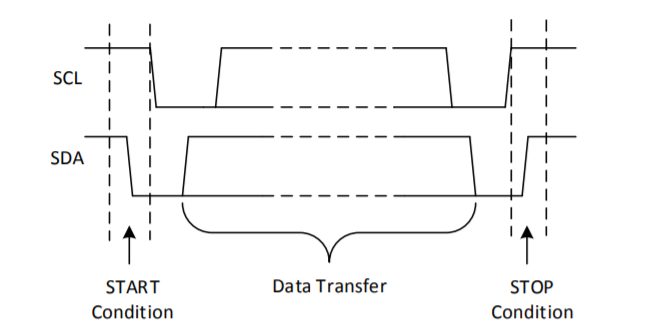
\includegraphics[scale=0.5]{images/start-stop-condition.png}
	\end{figure*}
	Start condition is happend when SDA line goes low from high while SCL is high. SDA line going high to low while SCL is high defines STOP condition.
\end{itemize}

\subsection{Sending data from master to slave}
\begin{figure*}[h!]
	\centering
	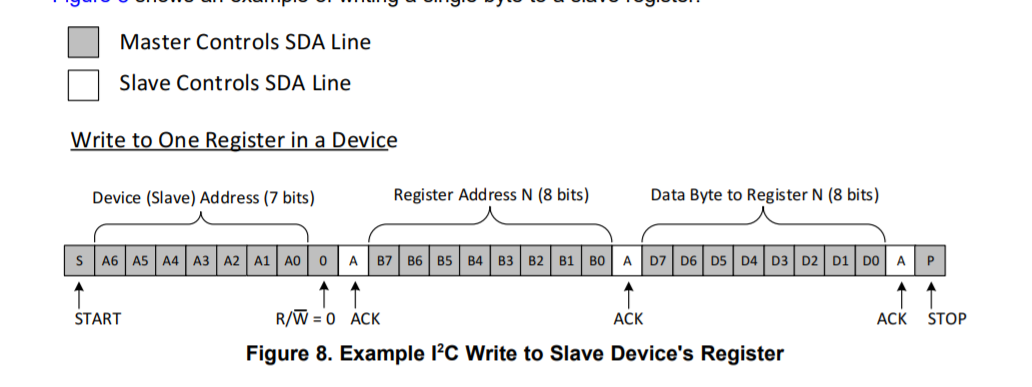
\includegraphics[scale=0.5]{images/master-write.png}
\end{figure*}
Master first send start condition followed by slave devices address and $R/\tilde{W}$ bit which is 0 this time.
Then if slave is ready to communicate then it sends acknowledge (ACK) signal. 
Then Master sends 8 bit data. Then slave sends ACK signal. Again master sends 8 bit data and slave reply with ACK bit. If slave unable to send ACK bit then error happens and master send stop condition and report error.

\subsection{Receiveing data from slave to master}
'\begin{figure*}[h!]
	\centering
	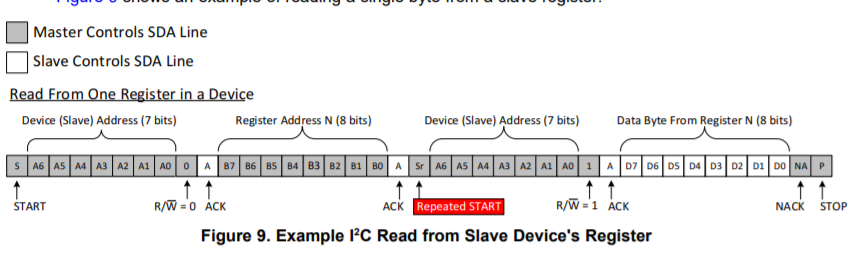
\includegraphics[scale=0.53]{images/master-read.png}
\end{figure*}

Slave cannot send start condition. If slave needs to transmit data to master then master needs to start connection and make $R/\tilde{W}$ bit to 1. 
Master release control of sda line when data should be written by slave.
Master always send clock pulse to SCL line irrespective of $R/\tilde{W}$ bit. 
After slave write data , then master sends NACK signal to sda line. 



\section{Advantages of TWI/I2C}

\begin{itemize}
	\item I2C uses only two wires whereas,
	 SPI uses atleast 2 wires for simplex communcation and 3 wires for duplex communication . 
	 \item Supports multiple master and multiple slaves. But USART works with only two devices.
	 \item ACK/NACK confirms successful data transfer.
	 \item TWI offers multiple master/slave support which UART does not.
	 \item Faster than UART
\end{itemize}

\section{Disadvantages of TWI/I2C}

\begin{itemize}
	\item Connection is half duplex , SPI or USART is full duplex.
	\item Size of data frame is only 8 bit and cannot be changed.
	 In USART communcation size of data frame can be choosen from between 8 and 9 bit.
	\item More complicated hardware needed to implement than SPI
	\item Slower transfer rate then SPI.
\end{itemize}

\section{References}

\end{document}